% Created 2021-08-20 Fri 17:03
% Intended LaTeX compiler: pdflatex
\documentclass[11pt]{article}
\usepackage[utf8]{inputenc}
\usepackage[T1]{fontenc}
\usepackage{graphicx}
\usepackage{grffile}
\usepackage{longtable}
\usepackage{wrapfig}
\usepackage{rotating}
\usepackage[normalem]{ulem}
\usepackage{amsmath}
\usepackage{textcomp}
\usepackage{amssymb}
\usepackage{capt-of}
\usepackage{hyperref}
\author{Anand Deopurkar}
\date{\today}
\title{Error correcting codes\\\medskip
\large How to talk across a noisy room?}
\hypersetup{
 pdfauthor={Anand Deopurkar},
 pdftitle={Error correcting codes},
 pdfkeywords={},
 pdfsubject={},
 pdfcreator={Emacs 27.1 (Org mode 9.3.7)}, 
 pdflang={English}}
\begin{document}

\maketitle

\section*{Noisy communication channels}
\label{sec:org1ce0c8a}
\subsection*{Is this working?}
\label{sec:orgdff14f5}
\href{isthisworking.png}{
\includegraphics[width=.9\linewidth]{/home/anandrd/website/talks/extension/isthisworking.png}}

\subsection*{Am I muted?}
\label{sec:org90cb712}
\href{muted.png}{
\includegraphics[width=.9\linewidth]{/home/anandrd/website/talks/extension/muted.png}}
\subsection*{Can you hear me through space?}
\label{sec:orgc01e9b4}
\href{rover.jpg}{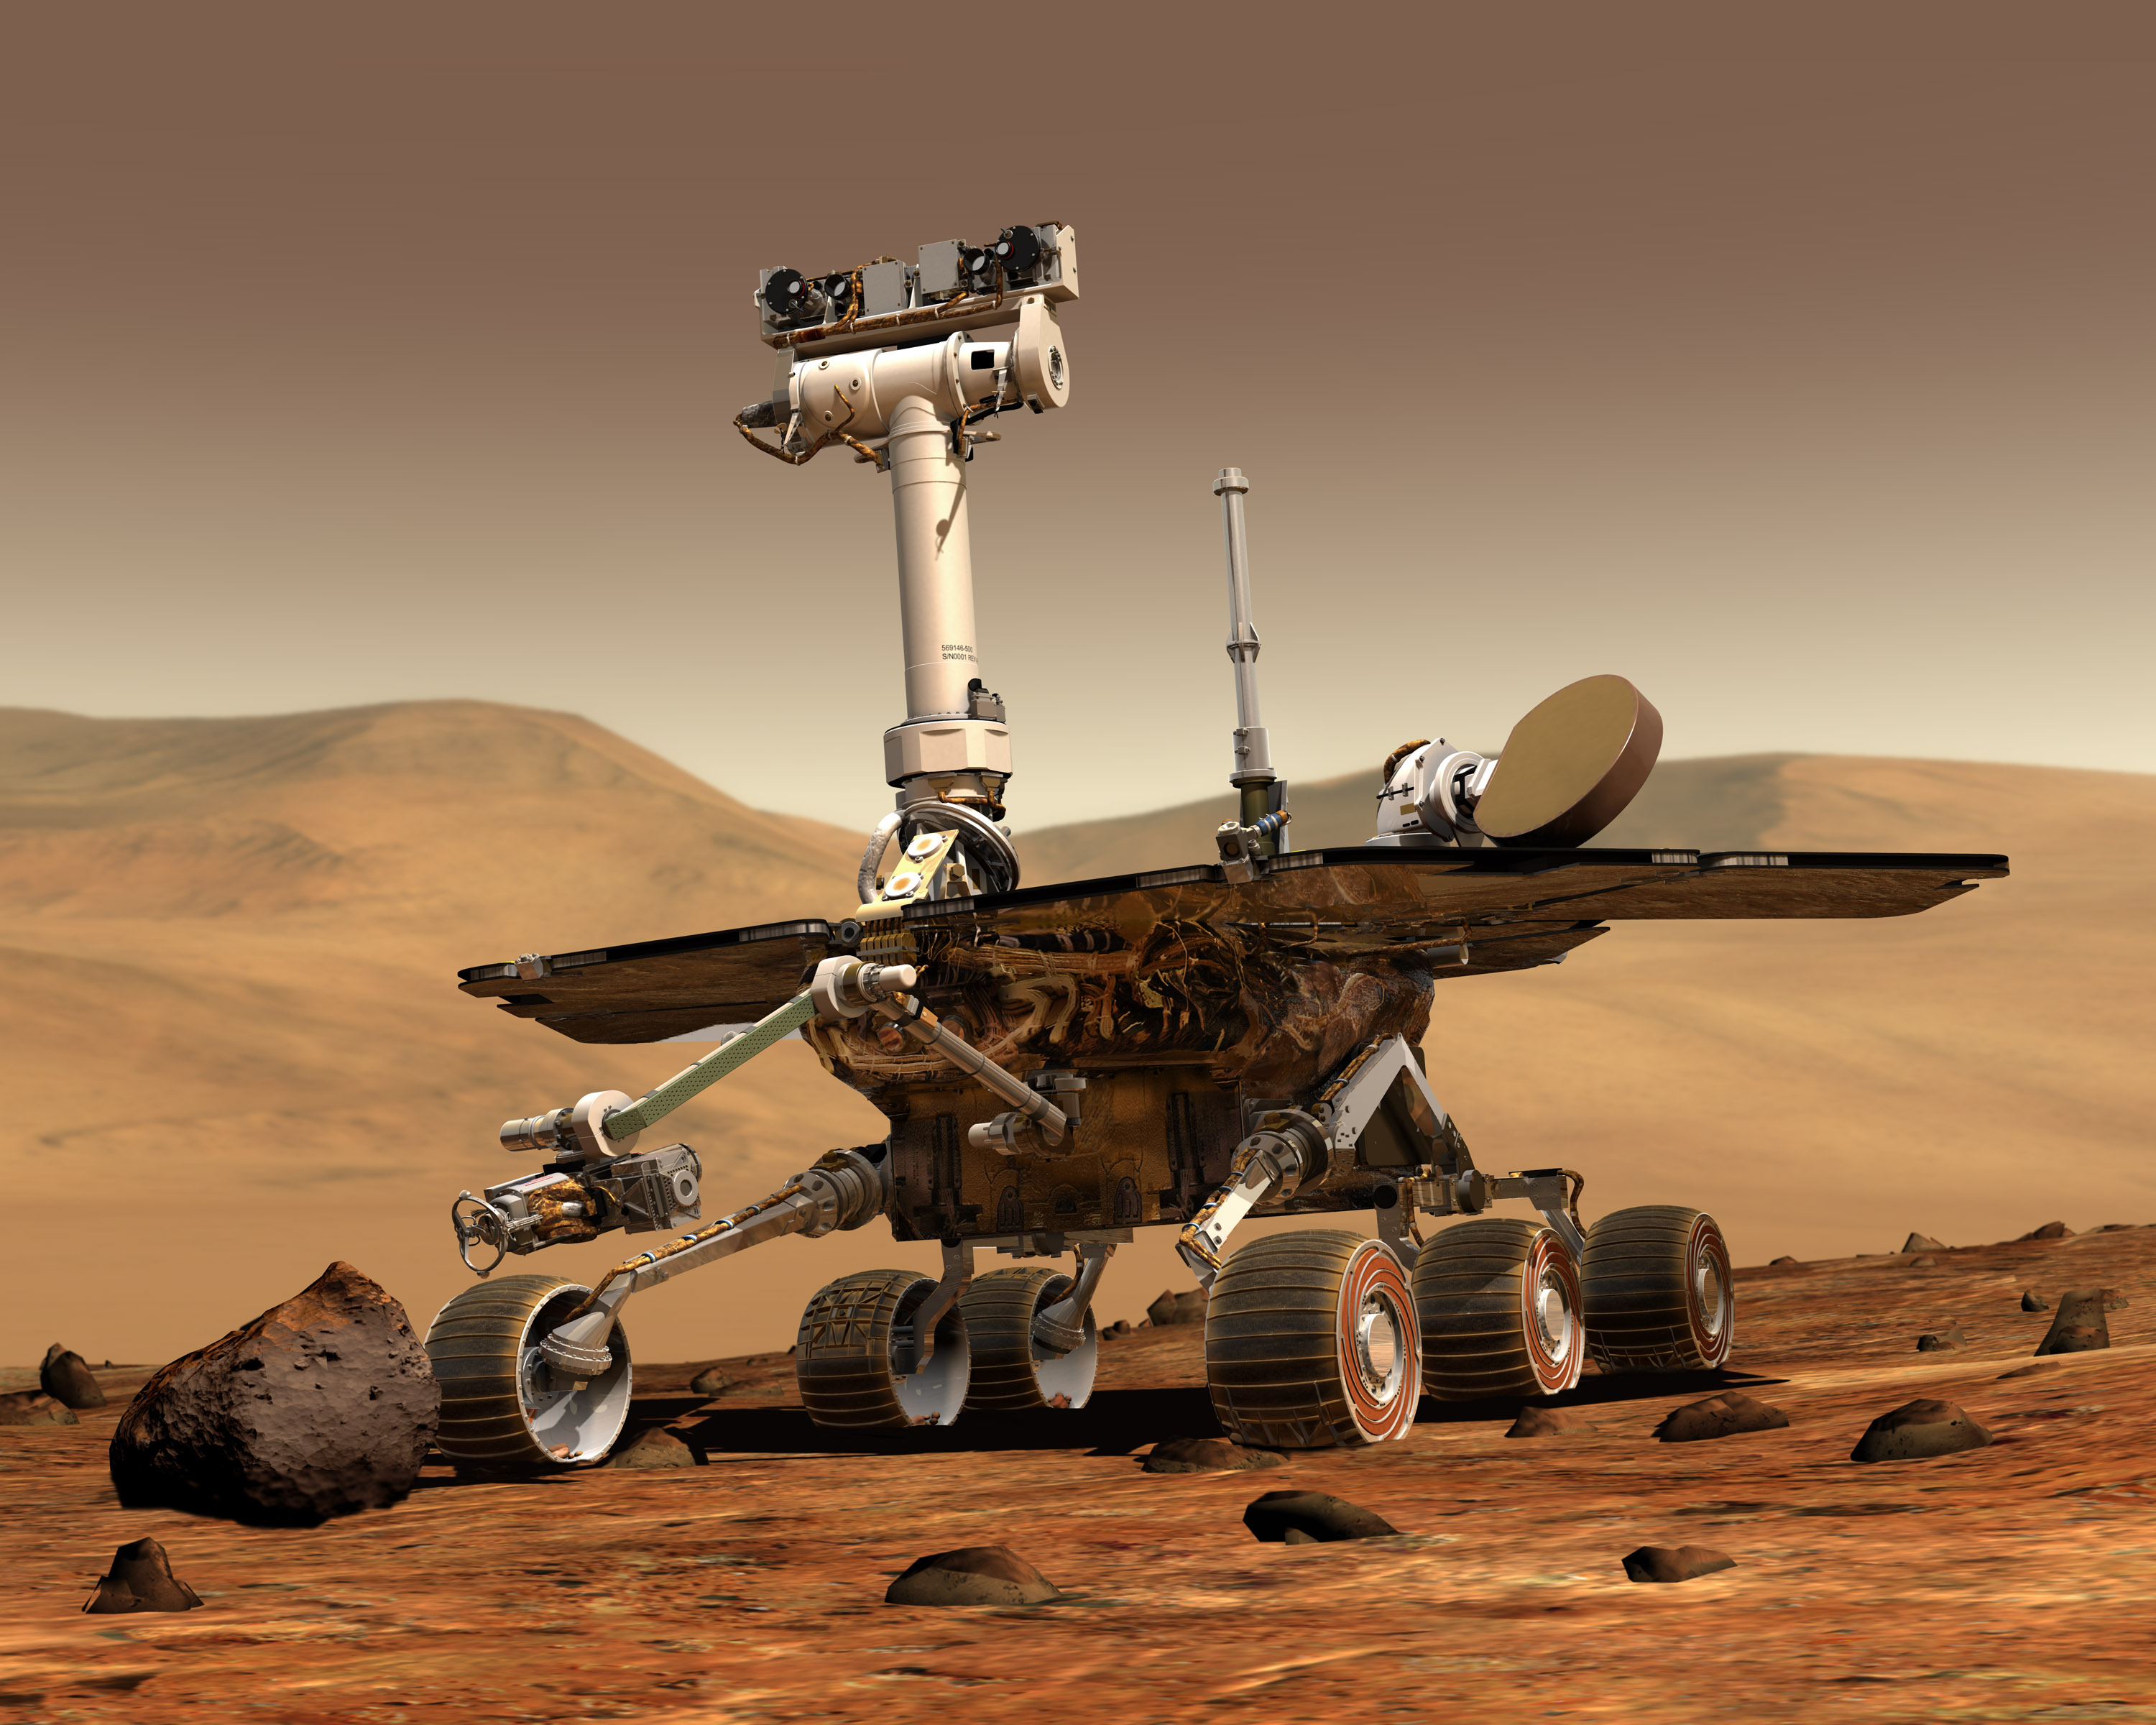
\includegraphics[width=.9\linewidth]{/home/anandrd/website/talks/extension/rover.jpg}}

\subsection*{Can you hear me through the atmosphere?}
\label{sec:org6251ae1}
\href{satellite.jpg}{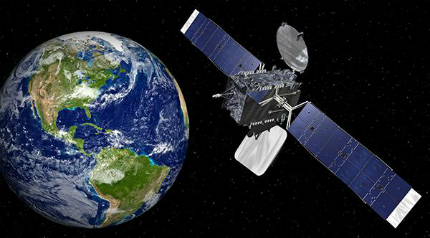
\includegraphics[width=.9\linewidth]{/home/anandrd/website/talks/extension/satellite.jpg}}

\section*{Errors are inevitable}
\label{sec:orgdc0c07a}
\begin{center}

\includegraphics[width=.9\linewidth]{canyouhearme.jpg}
\end{center}

\href{monkeywords.svg}{\includesvg[width=.9\linewidth]{/home/anandrd/website/talks/extension/monkeywords}}

\begin{center}
\includesvg[width=.9\linewidth]{monkeycode}
\end{center}

\section*{Correcting errors}
\label{sec:orgc9b7313}
\begin{center}
\includesvg[width=.9\linewidth]{monkeycorrection}
\end{center}

\section*{Can we do better?}
\label{sec:orgea2f297}
Yes, we can.

Using number theory!

\section*{The strategy}
\label{sec:org0b12d55}
We have a set \(M\) of messages (strings of length \(n\)).

We encode each \(m \in M\) to a longer string \(f(m)\).

So that \(f(m_1)\) and \(f(m_2)\) are not too close if \(m_1 \neq m_2\).

\subsection*{What is "too close"?}
\label{sec:org290d20e}
Given two strings \(n_1\) and \(n_2\), define the \emph{Hamming distance} \(d(n_1,n_2)\)between them to be the number of places in which \(n_1\) and \(n_2\) differ.

Not too close = Hamming distance at least \(k\).

\subsection*{Using the strategy}
\label{sec:org0fe615c}
\begin{center}
\includesvg[width=.9\linewidth]{monkeystrategy}
\end{center}

Allows \(\lfloor k/2 \rfloor\) errors to be corrected!

Allows \(\lfloor k/2 \rfloor\) errors to be corrected!

\begin{center}
\includesvg[width=.9\linewidth]{monkeyhamming}
\end{center}

\section*{How we execute the strategy?}
\label{sec:org65f95d1}

How do we find an \(f\)?

Using finite fields!

\section*{What is a field?}
\label{sec:orgcc53245}

A field \(F\) is a set together with operations \(+\) (addition) and \(\times\) (multiplication) satisfying the familiar rules.

\begin{enumerate}
\item Addition is associative, commutative, has an identity element (\(0\)).
\item Multiplication is associative, commutative, has an identity element (\(1\)).
\item Distributive law holds: \(a \times (b+c) = a \times b + a \times c\).
\item Every non-zero element has a multiplicative inverse.
\end{enumerate}

\subsection*{Examples}
\label{sec:orgfa0d09b}
\begin{enumerate}
\item \(\mathbb Q\) is a field (with the usual \(+, \times\)).
\item \(\mathbb R\) is a field (with the usual \(+, \times\)).
\end{enumerate}

\subsection*{Finite fields}
\label{sec:org47a59ac}
Take \(\mathbb F_p = \{0,1,\dots, p-1\}\)\\
with \(+\) and \(\times\) done modulo \(p\).

Theorem: \(\mathbb F_p\) is a field.


Multiplicative inverses in \(\mathbb F_5\).
   \begin{align*}
\overline{1}^{-1} &= \overline 1 \\
\overline{2}^{-1} &= \overline 3, \quad \overline{3}^{-1} = \overline 2 \\
\overline{4}^{-1} &= \overline 4
   \end{align*}

\subsection*{Polynomials}
\label{sec:orgb5f03d1}
For any field \(F\), let \(F[x]\) denote the set of polynomials with variable \(x\) and coefficients in \(F\).

Example: In \(\mathbb F_5[x]\), we have elements like
\begin{align*}
 \overline 0,\\
 \overline 2 \cdot x + \overline 1, \\
 \overline 1 \cdot x^2 + \overline 3 \cdot x + \overline 2.
\end{align*}

We add and multiply polynomials as usual, but remembering to always use the given operations for \(F\).

For example, in \(\mathbb F_5[x]\), we have
\[
   (\overline 2 x+ \overline 1) \cdot (\overline 1 x+ \overline 3) = \overline 2 x^2 + \overline 2 x + \overline 3.
   \]

\subsection*{Zeros of polynomials}
\label{sec:org0a4d66b}
Most of the usual properties of polynomials continue to hold.

\begin{enumerate}
\item If \(p(a) = 0\) then \((x-a)\) divides \(p(x)\); that is, \(p(x) = (x-a) q(x)\) for some \(q(x)\).
\item As a result, if \(p(x)\) has degree \(n\), then it has \emph{at most \(n\) zeros.}
\item As a result, if \(p_1(x)\) and \(p_2(x)\) are distinct and have degree at most \(n\), then \(p_1(a) = p_2(a)\) for \emph{at most \(n\) values of \(a\)}.
\end{enumerate}

\section*{Reed-Solomon codes}
\label{sec:org89cfede}
Message space: length-3 strings of \(\{0,1,2,3,4\}\).

Encoding \((p_1, p_2, p_3)\)
\begin{enumerate}
\item Think of \((p_1,p_2,p_3)\) as the polynomial \(p(x) = p_1 x^2 + p_2 x + p_3\) in \(\mathbb F_5[x]\).
\item Encode this polynomial into a length-5 string \((p(0),p(1),p(2),p(3),p(4))\).
\end{enumerate}

\begin{enumerate}
\item Think of \((p_1,p_2,p_3)\) as the polynomial \(p(x) = p_1 x^2 + p_2 x + p_3\) in \(\mathbb F_5[x]\).
\item Encode this polynomial into a length-5 string \((p(0),p(1),p(2),p(3),p(4))\).
\end{enumerate}

Example:
\begin{align*}
(1,1,1) &\mapsto {\small (0^2+0+1, 1^1+1+1, 2^2+2+1, 3^2+3+1, 4^2+4+1)} \\
&== (1,3,2,3,1).
\end{align*}

\subsection*{What is the hamming distance?}
\label{sec:org91224a6}
What is the Hamming distance of the encodings of \(p\) and \(q\)?

At least 3!

Two distinct polynomials of degree at most 2 \emph{must differ} in at least 3 out of the 5 values of \(x\) in \(\mathbb F_5\).

\subsection*{Recap}
\label{sec:orgbe47483}
Encode: Length-3 string to length-5 string

Gain: Ability to correct any 1-bit errors.

Better than tripling!

\section*{Applications}
\label{sec:orgaec01ea}
Reed-Solomon codes (and their more sophisticated analogues) are used in many places!

\begin{center}
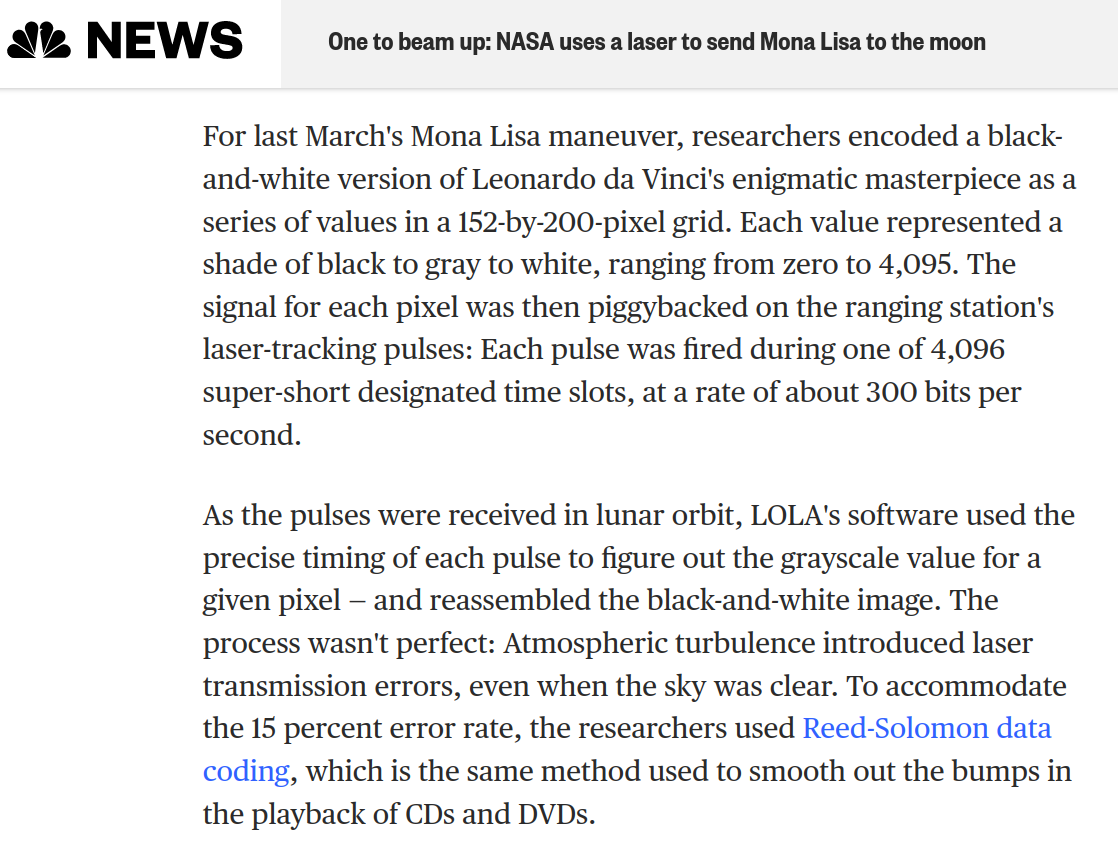
\includegraphics[width=.9\linewidth]{news.png}
\end{center}

\begin{center}
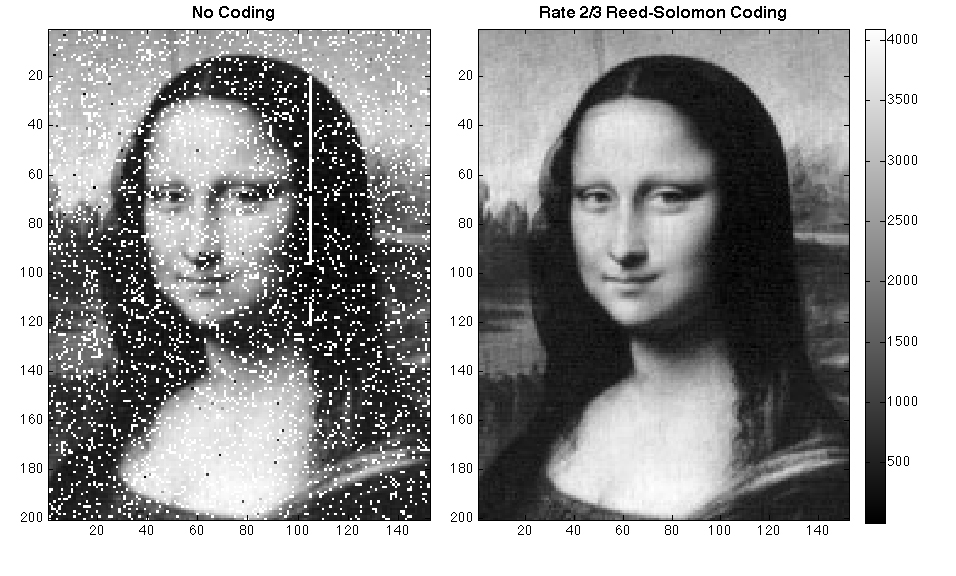
\includegraphics[width=.9\linewidth]{monalisa.jpg}
\end{center}

\begin{center}
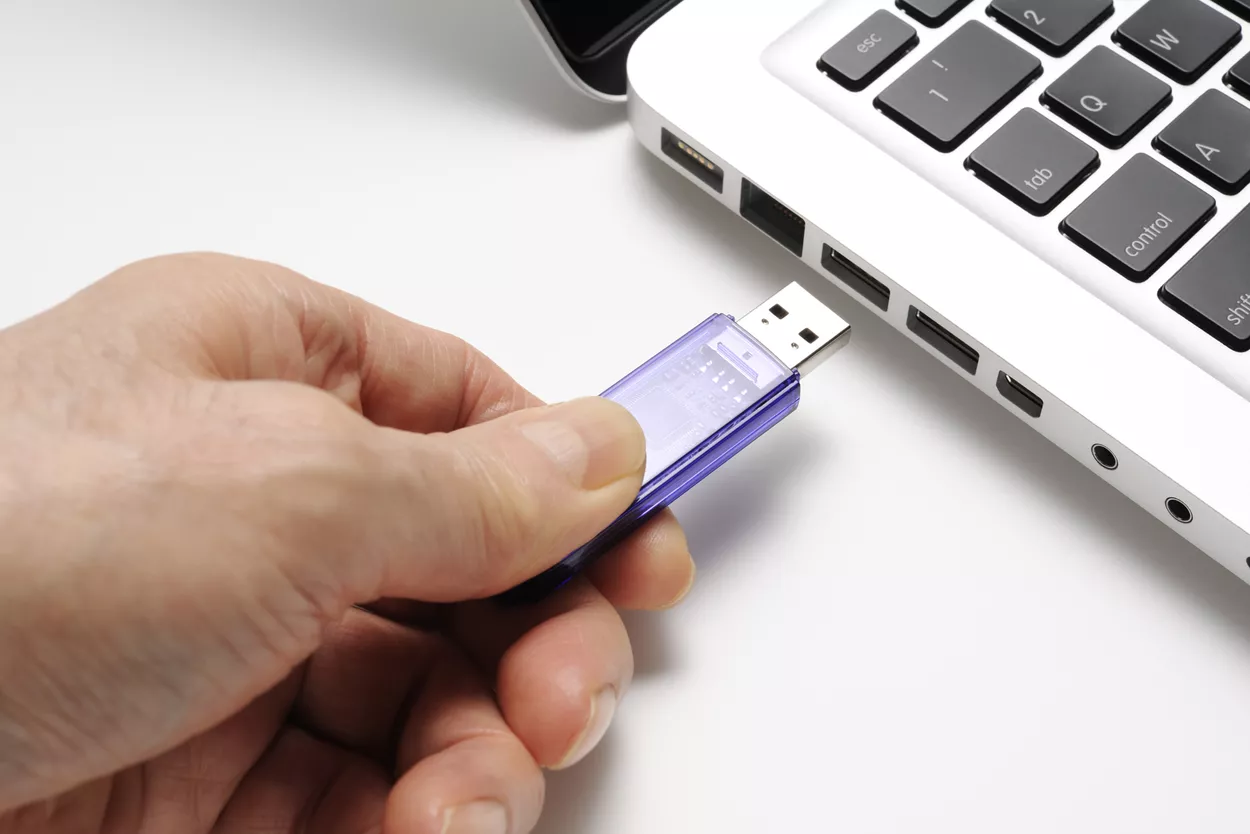
\includegraphics[width=.9\linewidth]{flashdrive.png}
\end{center}

\begin{center}
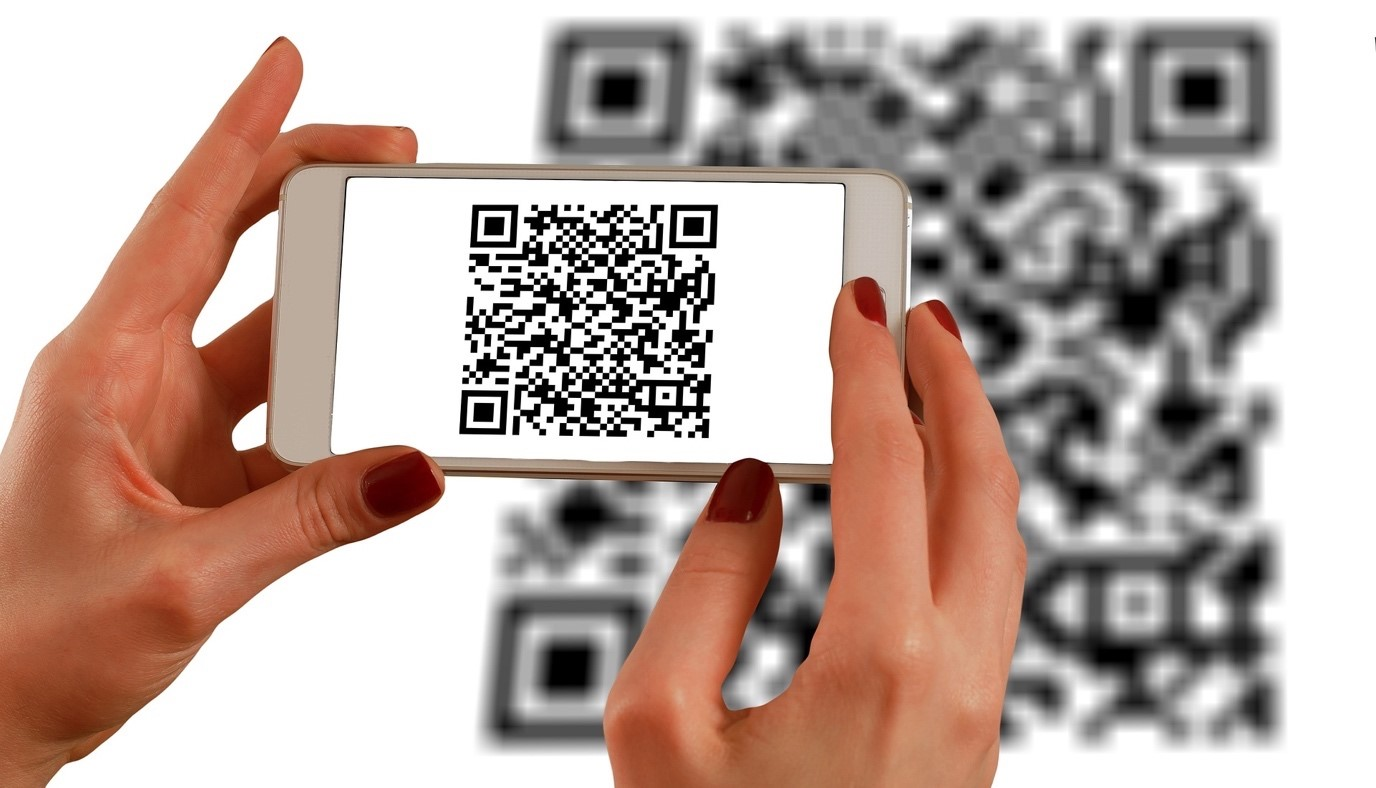
\includegraphics[width=.9\linewidth]{qr.jpg}
\end{center}

\section*{More questions}
\label{sec:orge26d810}

\begin{enumerate}
\item Are there other finite fields, besides \(\mathbb F_p\)?
\item Can we do better than Reed-Solomon?
\end{enumerate}

\section*{Thank you!}
\label{sec:org32f9861}
\end{document}